\documentclass[12pt,letterpaper]{article}

\usepackage{fancyhdr}
\pagestyle{fancy}
\fancyhf{}
\rhead{Vaja 6}
\lhead{ORS}
\setlength{\headheight}{16pt}

\usepackage[utf8]{inputenc}
\usepackage[slovene]{babel}
\usepackage[colorlinks = true, urlcolor = blue]{hyperref}

\usepackage{xcolor}
\usepackage{listings}
\usepackage{graphicx}
\graphicspath{{./images/}}
\definecolor{mGreen}{rgb}{0,0.6,0}
\definecolor{mGray}{rgb}{0.5,0.5,0.5}
\definecolor{mPurple}{rgb}{0.58,0,0.82}
\definecolor{backgroundColour}{rgb}{1,1,1}

\lstdefinestyle{CStyle}{
    backgroundcolor=\color{backgroundColour},   
    commentstyle=\color{mGreen},
    keywordstyle=\color{magenta},
    numberstyle=\tiny\color{mGray},
    stringstyle=\color{mPurple},
    basicstyle=\footnotesize,
    breakatwhitespace=false,         
    breaklines=true,                 
    captionpos=b,                    
    keepspaces=true,                 
    numbers=left,                    
    numbersep=5pt,                  
    showspaces=false,                
    showstringspaces=false,
    showtabs=false,                  
    tabsize=2,
    language=C,
    frame=none
}

\begin{document}

\begin{center}
    \textbf{\Large Izjeme, prekinitve ter zunanje prekinitve v STM32F4 (Cortex-M)}   
\end{center}

\subsection*{Izjeme (angl. exceptions)}

Izjeme (angl. exceptions) so dogodki, ki lahko prekinejo centralno procesno enoto med izvajanjem nekega programa ali niza ukazov z namenom izvedbe niza ukazov, ki izjemo servisira. Odločitev o tem, ali bo določena izjema dejansko prekinila izvajanje je odvisna od tega kakšno prioriteto imata izjema ter program, ki ga izjema prekinja. V primeru, da ima izjema višjo prioriteto, se zgodi servisiranje izjeme, v nasprotnem primeru pa izjema čaka dalje. Obstaja več tipov izjem, ki jih bomo spoznali v nadaljevanju. 

\subsection*{Prekinitve (angl. interrupts)}

Najpogosteje se srečujemo s tipom izjem, ki jim rečemo prekinitve. Prekinitve so izjeme, ki jih dvignejo periferne naprave, da sporočijo centralni procesni enoti (CPE), da se je zgodilo nekaj, kar bi CPE znalo ``zanimati``. Primeri so:

\begin{itemize}
    \item pritisk gumba,
    \item senzor je zaznal prosti pad,
    \item temperaturni senzor je zaznal visoko temperaturo,
    \item vezje za branje stanja baterije je zaznalo, da je baterija prazna,
    \item zaznan je bil klik na zaslonu na dotik,
    \item senzor gibanja je zaznal gibanje.
\end{itemize}

Poleg omenjenih izjem med prekinitve štejemo tudi dve prekinitvi, ki se prožita znotraj procesorja. Prva je \texttt{SysTick}, ki jo periodično generira sistemski časovnik. To prekinitev pogosto uporabljajo operacijski sistemi za merjenje časovnih rezin in preklapljanje opravil. Tudi funkcija \texttt{HAL\_Delay()}, ki ste jo že uporabili na preteklih vajah, se zanaša na omenjeno prekinitev.

Druga prekinitev, ki se generira znotraj procesorja je \texttt{PendSV}, to prekinitev prožimo programsko in se jo uporablja za preklop konteksta (angl. context switch) v večopravilnih operacijskih sistemih.

Poznamo še posebno vrsto prekinitev, ki se imenuje ne-maskirajoče prekinitve (angl. non-maskable interrupt). Te so posebne v tem, da imajo izjemno visoko prioriteto, ki jo presega zgolj reset, kar pomeni da bodo praktično vedno prekinile trenutno izvajajoči proces.

\subsection*{Napake (angl. fault)}

Napake so posledica neobičajnih dogodkov, ki jih zazna procesor. Ti dogodki so lahko notranji na primer napake med komunikacijo s pomnilnikom ali drugimi napravami. Napake običajno signalizirajo resne težave v strojni ali programski opremi, ki onemogočajo normalno izvajanje programa. Poznamo sledeče napake:

\begin{itemize}
    \item \textbf{UsageFault} napaka, ki se sproži, ko ukaza ne moremo izvesti. Bodisi ker ukaz ni definiran ali ga ni možno izvesti. Primer bi bilo deljenje z ničlo.
    \item \textbf{BusFault} se proži ob napaki na ukaznem ali podatkovnem vodilu ob dostopu do pomnilnika.
    \item \textbf{MemManage} se proži ob dostopu do zaščitenega dela pomnilnika.
    \item \textbf{HardFault} se proži, če do napake pride med servisiranjem drugih izjem. Pod posebnimi pogoji lahko tudi ostale izjeme eskalirajo v napako tipa HardFault.
\end{itemize}

Do eskalacije napak v HardFault pride, ko se napaka pripeti v funkcijah, ki servisirajo izjeme z enako ali višjo prioriteto (v tem primeru se napaka ne bi servisirala) ali pa se zgodi napaka za katero ni definirane funkcije, ki se v tem primeru izvede.

\subsection*{Nadzorni klic (angl. supervisor call)}

Ta izjema se pripeti ob izvedbi posebnega supervisor call (SVC) ukaza. Ti se uporabljajo kot priročen način, da običajni programi zahtevajo, da jedro operacijskega sistema (angl. operating system kernel) izvede določene funkcije v njihovem imenu. S pomočjo tega ukaza lahko naši mikrokrmilniški programi, ki tečejo v nepriviligiranih načinih, dobijo dostop do posebnih registrov za katere sicer nimajo zadosti pravic.

\subsection*{Reset}

Posebna izjema je \texttt{reset}, ki se pripeti ob vsakem vklopu procesorja ter v primeru tako imenovanega toplega reseta (angl. warm reset). Tega na naših razvojnih ploščah dosežemo s pritiskom črne (reset) tipke. Ta izjema je posebna v tem, da lahko prekine delovanja v vsakem primeru. Razlikuje se tudi v načinu delovanja, kar bomo spoznali v nadaljevanju.


\section*{Prioritete izvajanj}

V mikrokrmilnikih Cortex-M, med katere spada tudi STM32F4, so prioritete označene s celimi števili, nižje število pa pomeni višjo prioriteto. Najvišjo prioriteto z vrednostjo -3 ima izjema \texttt{Reset}. Sledijo ne-maskirajoče prekinitve (NMI) s prioriteto -2 in \texttt{HardFault} s prioriteto -1. Ostale izjeme imajo programsko nastavljivo prioriteto med 0 in 255.

Ko pride do izjeme se bo ta servisirala v primeru, da je njena prioriteta nižja od trenutne prioritete izvajanja. Osnovna prioriteta izvajanega programa je 256. V primeru, da se izvaja servisiranje izjeme je prioriteta izvajanega programa enaka prioriteti izjeme. Osnovno prioriteto lahko spremenimo z vpisom vrednosti v poseben register \texttt{BASEPRI}. Če v ta register vpišemo vrednost 5, bo to pomenilo, da se bodo lahko servisirale zgolj izjeme, ki imajo višjo prioriteto od 5 (-3, -2, -1, 0, 1, 2, 3 ali 4). 
Poleg priororitete imamo za nadziranje izjem in prekinitev še dva dodatna enobitna registra, ki določene izjeme maskirata (onemogočita). V primeru, da je postavljen bit 0 v registru \texttt{PRIMASK} je najnižja prioriteta izvajanega programa 0. To pomeni, da se bodo servisirale zgolj izjeme \texttt{HardFault}, \texttt{NMI} in \texttt{Reset}.

V primeru, da je postavljen bit 0 v registru \texttt{FAULTMASK} je najnižja prioriteta izvajanega programa -1. To pa pomeni, da se bodo servisirale zgolj izjeme \texttt{NMI} in \texttt{Reset}. Grafični prikaz mehanizma za prioriteta je prikazan na sliki \ref{prioriteta}. 

\begin{figure}[ht!]
  \centering
  \caption{Mehanizem za upravljanje s prioriteto izjem.}
  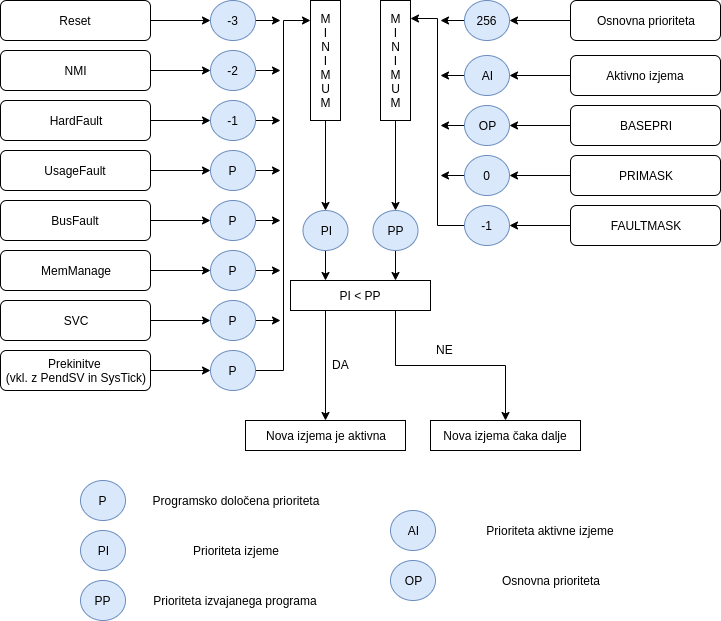
\includegraphics[width=360pt]{images/vaja6/prioriteta.png}
  \label{prioriteta}
\end{figure}

\newpage


\section*{Načini delovanja}

Mikrokrmilniki iz družine Cortex-M imajo 2 načina delovanja: Thread in Handler. Razlika med njima je v pravicah dostopa do posebnih registrov mikrokrmilnika (npr. CONTROL). V Handler način delovanja centralna procesna enota preklopi kadar servisira izjeme. Edina izjema, za katero to ne drži, je \texttt{Reset}, servisiranje te izjeme se namreč izvaja v Thread načinu.
Prav tako je pogosto razlika med načini delovanja tudi v skladovnem kazalcu, ki se med servisiranjem uporablja. Tega, tako kot običjano hranimo v registru \texttt{r13}. V Handler načinu se uporabi glavni skladovni kazalec (angl. Main Stack pointer - MSP), v Thread načinu pa procesni skladovni kazalec (angl. Process Stack Pointer - PSP). 

\section*{Preklop v servisiranje izjeme}

V primeru, da ima izjema, ki se pojavi, dovolj visoko prioriteto, da postane aktivna, se začne servisiranje izjeme. Preklop v servisiranje izjeme je prikazan na sliki \ref{contextSwitch}. Najprej se shrani del stanja (konteksta) procesorja na sklad. Shranijo se programski števec (angl. program counter - PC), register za povratni naslov (angl. link register - LR), statusni register (angl. program status register - xPSR) ter splošno-namenski registri R0, R1, R2, R3 in R12. Procesor ima na voljo dva sklada in posledično dva skladovna kazalca, glavni skladovni kazalec (MSP) ter procesni skladovni kazalec (PSP). Običajno se uporabi glavni skladovni kazalec, razen če programsko določimo drugače.

\begin{figure}[ht!]
  \centering
  \caption{Preklop v servisiranje izjeme.}
  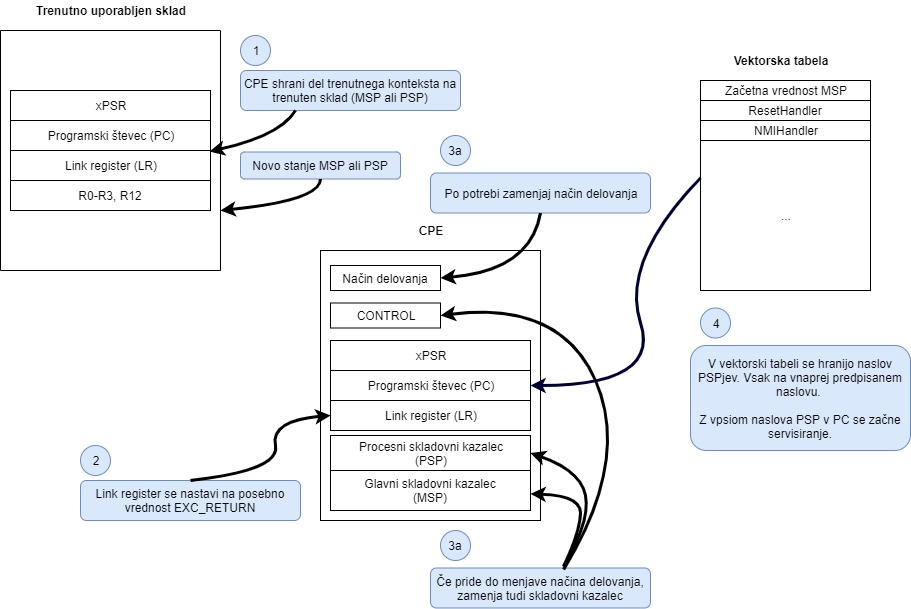
\includegraphics[width=390pt]{images/vaja6/contextswitch.jpg}
  \label{contextSwitch}
\end{figure}

Po shranjevanju na sklad se v LR zapiše posebna vrednost, ki jo ARM označuje kot \texttt{EXC\_RETURN}. V primeru, da je potrebno, sledi preklop načina delovanja in menjava skladovnega kazalca. Hkrati se v register \texttt{IPSR} shrani oznaka izjeme. Zadnji korak preklopa v servisiranje izjeme je nastavljanje programskega števca iz vektorske tabele. Kateri vnos iz vektorske tabele procesor vzame je odvisno od oznake izjeme. Prvi vnos v vektorski tabeli pripada začetnemu naslovu funkcije, ki servisira \texttt{Reset} izjemo. Sledi začetni naslov funkcije za servisiranje ne-maskirajočih prekinitev, in tako dalje. Vektorska tabela se nahaja na začetku pomnilniškega prostora, pred njo se nahaja zgolj začetna vrednost glavnega skladovnega kazalca. Vektorska tabela se v projektu za STM32CubeIDE nahaja v \texttt{Startup/startup\_stm32f407vgtx.s}. Izsek vektorske tabele je prikazan spodaj.

\begin{center}
\begin{lstlisting}[style=CStyle]
g_pfnVectors:
  .word  _estack
  .word  Reset_Handler
  .word  NMI_Handler
  .word  HardFault_Handler
  .word  MemManage_Handler
  .word  BusFault_Handler
  .word  UsageFault_Handler
  .word  0
  .word  0
  .word  0
  .word  0
  .word  SVC_Handler
  .word  DebugMon_Handler
  .word  0
  .word  PendSV_Handler
  .word  SysTick_Handler
  
  /* External Interrupts */
  .word     WWDG_IRQHandler                               
  .word     PVD_IRQHandler
  .word     TAMP_STAMP_IRQHandler
  .word     RTC_WKUP_IRQHandler
  .word     FLASH_IRQHandler            
  .word     RCC_IRQHandler                
  .word     EXTI0_IRQHandler
  .word     EXTI1_IRQHandler
  .word     EXTI2_IRQHandler
  .word     EXTI3_IRQHandler
  .word     EXTI4_IRQHandler
\end{lstlisting}
\end{center}
Psevdoukaz \texttt{.word} označuje, da na tem mestu shranjujejmo 32-bitno vrednost. Kot vrednosti so zapisana imena podprogramov v zbirniku ali funkcij v C-ju. Ime funkcije pa je dejansko naslov začetka funkcije, podobno kot ime polja predstavlja naslov začetka polja.

Prva vrstica vektorske tabele označuje začetno vrednost glavnega skladovnega kazalca MSP. Sledi oznaka \texttt{Reset\_Handler}. Ta pomeni, da se bo v primeru, da pride do izjeme \texttt{Reset}, izvedla funkcija z imenom \texttt{Reset\_Handler}. Ta se nahaja v isti datoteki in je napisana v ARM zbirniku. Spodaj so navedena tudi imena funkcij, ki se bodo izvedle v primeru prekinitev. Tako funkcijo imenujemo prekinitveno servisni program (angl. interrupt request handler), zato se končajo s končnico \texttt{IRQHandler}. Za delo s prekinitvami je potrebno poznati tako oznake izjem kot imena prekinitveno servisnih programov. V \texttt{Drivers/CMSIS/Device/ST/STM32F4xx/Include/stm32f407xx.h} lahko najdete oznake izjem. Izsek oznak je prikazan spodaj.

\begin{center}
\begin{lstlisting}[style=CStyle]
typedef enum
{
/******  Cortex-M4 Processor Exceptions Numbers ****************************/
  NonMaskableInt_IRQn     = -14, /*!< 2 Non Maskable */
  MemoryManagement_IRQn   = -12, /*!< 4 Cortex-M4 Memory Management */
  BusFault_IRQn           = -11, /*!< 5 Cortex-M4 Bus Fault */
  UsageFault_IRQn         = -10, /*!< 6 Cortex-M4 Usage Fault */
  SVCall_IRQn             = -5, /*!< 11 Cortex-M4 SV Call */
  DebugMonitor_IRQn       = -4, /*!< 12 Cortex-M4 Debug Monitor */
  PendSV_IRQn             = -2, /*!< 14 Cortex-M4 Pend SV */
  SysTick_IRQn            = -1, /*!< 15 Cortex-M4 System Tick */
/******  STM32 specific Interrupt Numbers ************************/
  WWDG_IRQn         = 0, /*!< Window WatchDog Interrupt */
  PVD_IRQn          = 1, /*!< PVD through EXTI Line detection */
  TAMP_STAMP_IRQn   = 2, /*!< Tamper and TimeStamp interrupts */
  RTC_WKUP_IRQn     = 3, /*!< RTC Wakeup interrupt */
  FLASH_IRQn    = 4,      /*!< FLASH global Interrupt */
  RCC_IRQn      = 5,      /*!< RCC global Interrupt */
  EXTI0_IRQn    = 6,      /*!< EXTI Line0 Interrupt */
  EXTI1_IRQn    = 7,      /*!< EXTI Line1 Interrupt */
  EXTI2_IRQn    = 8,      /*!< EXTI Line2 Interrupt */
  EXTI3_IRQn    = 9,      /*!< EXTI Line3 Interrupt  */
  EXTI4_IRQn    = 10,     /*!< EXTI Line4 Interrupt  */
  ...
\end{lstlisting}
\end{center}

V datoteki \texttt{Src/stm32f4xx\_it.c} najdemo ogrodja servisnih funkcij za ostale napake. Za preostale izjeme je v datoteki definirano, da se v primeru, da ne obstaja funkcija z enakim imenom kot je definiran v vektorski tabeli, kliče funkcijo \texttt{Default\_Handler}. Ta je definirana v isti datoteki kot vektorska tabela, v njej je pa implementirana neskončna zanka.

V primeru, da želimo napisati prekinitveno servisni program za katero od preostalih izjem, moramo v eno izmed datotek projekta zapisati funkcijo z imenom, kot je zapisan v vektorski tabeli. Dobra praska je, da servisne programe izjem pišemo v datoteko \texttt{Src/stm32f4xx\_it.c}.

\subsection*{Prekinitveni krmilnik NVIC}

Vse prekinitve z izjemo prekinitev \texttt{SysTick} in \texttt{PendSV} do mikrokrmilnika pridejo iz zunanjih naprav. Vendar pa ne neposredno, temveč preko prekinitvenega krmilnika. Ta omogoča, da lahko vsak posamičen prekinitveni vir programsko vklopimo ali izklopimo ter mu določamo prioriteto. S knjižico STM32 HAL to storimo preprosto z dvema ukazoma, kot je prikazano spodaj.

\begin{center}
\begin{lstlisting}[style=CStyle]
// za prekinitveni vir dolocimo prioriteto
HAL_NVIC_SetPriority(RCC\_IRQn, 1, 2);

// vklopimo prekinitveni vir
HAL_NVIC_EnableIRQ(RCC\_IRQn); 
\end{lstlisting}
\end{center}

Prioriteto v prekinitvenem krmilniku določamo na dveh nivojih z vrednostmi od 0 do 15. Kot je bilo omenjeno na začetku tega dokumenta, to pomeni, da imamo skupaj 256 prioritetnih nivojev. Najprej se upošteva prioriteto na prvem nivoju in v primeru enakosti na prvem nivoju se naredi primerjava še na drugem nivoju.

Zadnji korak je, da dodamo prekinitveno servisni program za vklopljen prekinitveni vir. Za zgornji primer je to funkcija \texttt{RCC\_IRQHandler}.

\subsection*{Prekinitveno servisni programi}

Pri predmetu ORS bomo pisali predvsem prekinitveno servisne programe (PSP). Torej funkcije, ki servisirajo prekinitve. Bistveno pri PSP je, da v čim krajšem času odpravi razlog za prekinitev. Običajno je vsak PSP razdeljen v tri dele:

\begin{itemize}
    \item Preverjanje prekinitvenih virov: najprej moramo preveriti, da smo v PSP ravno zaradi izbranega prekinitvenega vira. To preverjamo tudi zato, ker je lahko isti PSP odgovoren za več prekinitvenih virov.
    
    \item Odpravljanje razloga za prekinitev.
    
    \item Brisanje prekinitvenih zahtev: pred izhodom iz PSP moramo obvezno poskrbeti, da je prekinitvena zahteva, ki smo jo pravkar servisirali, pobrisana.
\end{itemize}

\subsection*{Vračanje iz servisiranja izjem}

Po zaključku prekinitveno servisnih programov oziroma funkcij, procesor prebere vrednost shranjeno v regirstru \texttt{lr}. Če prebere prej omenjeno posebno vrednost \texttt{EXC\_RETURN}, ve da je funkcija, iz katere se vračamo, servisirala izjemo. Ob povratku v izvorni program preveri ali so izpolnjeni vsi pogoji za vračanje iz servisne funkcije, nato pa povrne stanje procesorja iz sklada. Povrnjeno stanje programskega števca tudi pomeni, da program nadaljuje na mestu kjer je bil prekinjen zaradi izjeme.

\section*{Zunanje prekinitve}

Prvi vir prekinitev, ki ga bomo podrobneje spoznali, so zunanje prekinitve (angl. external interrupts). To so prekinitveni viri, ki se uporabljajo predvsem za to, da lahko digitalni vhodni pini prožijo prekinitev. Tako bomo na primer znali doseči, da bo pritisk na gumb sprožil prekinitev.

Vhodni pini namreč sami ne morejo prožiti prekinitev preko GPIO naprave, ampak za to skrbi ločena naprava za zunanje prekinitve. Ta ima oznako EXTI. EXTI naprava omogoča zaznavo spremembe signala iz 0 v 1 (prva fronta, angl. rising edge) ali iz 1 v 0 (zadnja fronta, angl. falling edge) in proženje prekinitev ob zaznavanju ene ali obeh front.

Naprava EXTI ima 23 vhodnih linij, ki lahko prožijo prekinitve. Nas bodo zanimale predvsem linije 0 do 15. Na linijo 0 so namreč priklopljeni vsi pini z oznako Px0 (PA0, PB0, PC0, PD0, ...), na linijo ena vsi pini z oznako Px1, in tako naprej do linije 15. Pini so na EXTI linijo priklopljeni preko multiplekserjev prikazanih na sliki \ref{EXTImux}.

\begin{figure}[ht!]
  \centering
  \caption{Multiplekserji na vhodnih linijah EXTI.}
  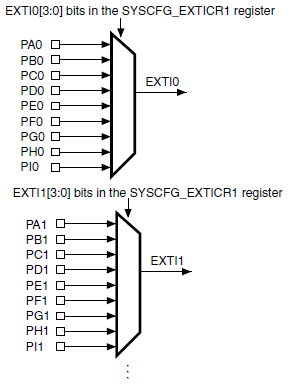
\includegraphics[width=120pt]{images/vaja6/mux.png}
  \label{EXTImux}
\end{figure}

Izhodi iz multiplekserjev so vhod v vezje na sliki \ref{exti}. Na levi strani vidimo, da je izhod iz vezja povezan na NVIC. Izhod vezja predstavlja stanje registra \texttt{Pending request register}. Ta register se nastavlja iz izhoda AND vrat. Ta je torej aktiven, ko sta oba vhoda aktivna. Prvi je \texttt{Interrupt mask register}, drugi pa izhod iz OR vrat. Če je bit v Interrupt mask register postavljen na 0, s tem onemogočimo, da bi linija prožila prekinitev. Ne glede na to kaj je na drugem vhod IN vrat, če je eden izmed vhodov nič, bo namreč izhod IN vrat vedno logična ničla. V primeru, da je bit v \texttt{Interrupt mask register} postavljen, pa za proženje prekinitve potrebujemo še logično enico iz OR vrat. To dobimo na dva načina. Prvi je, da postavimo bit v \texttt{Software interrupt event register}, ki omogoča programsko proženje EXTI prekinitev. Drugi način, ki je tudi tisti, ki bo nam prišel prav, je da vezje za zaznavanje fronte (angl. Edge detect circuit) zazna fronto na vhodnem signalu. To je tudi primarna funkcija EXTI naprave.

\begin{figure}[ht!]
  \centering
  \caption{EXTI naprava.}
  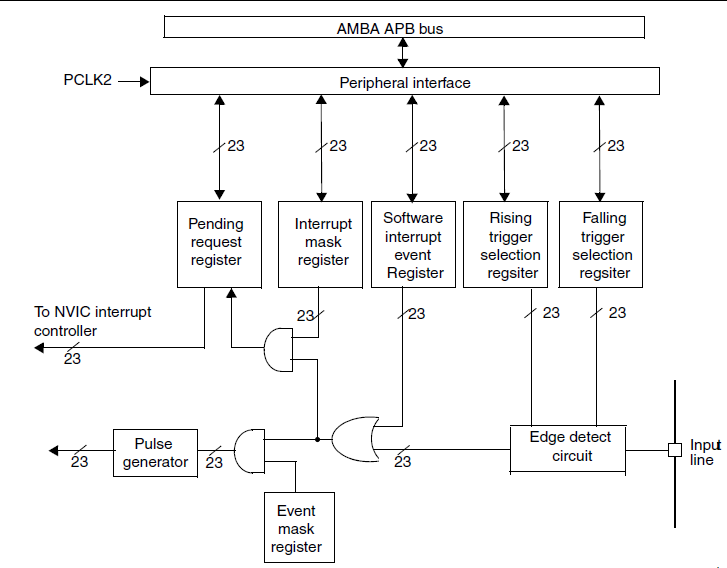
\includegraphics[width=300pt]{images/vaja6/exti.png}
  \label{exti}
\end{figure}

V tabeli \ref{EXTIIRQn} so zapisane prekinitvene oznake in imena prekinitveno servisnih programov vseh šestnajstih prekinitvenih linij, ki so vezane na GPIO pine.

\begin{table}[ht!]
\caption{Oznake prekinitvenih virov in imena PSP-jev.}
\begin{center}
\begin{tabular}{c|c|c}
\textbf{EXTI linija}   & \textbf{Oznaka prek. vira} & \textbf{Ime PSP-ja}             \\ \hline
EXTI0         & EXTI0\_IRQn       & EXTI0\_IRQHandler      \\ \hline
EXTI1         & EXTI1\_IRQn       & EXTI1\_IRQHandler      \\ \hline
EXTI2         & EXTI2\_IRQn       & EXTI2\_IRQHandler      \\ \hline
EXTI3         & EXTI3\_IRQn       & EXTI3\_IRQHandler      \\ \hline
EXTI4         & EXTI4\_IRQn       & EXTI4\_IRQHandler      \\ \hline
EXTI5 - EXTI9 & EXTI9\_5\_IRQn    & EXTI9\_5\_IRQHandler   \\ \hline
EXTI10-EXTI15 & EXTI15\_10\_IRQn  & EXTI15\_10\_IRQHandler \\
\end{tabular}
\label{EXTIIRQn}
\end{center}
\end{table}


\subsection*{Vklop prekinitev za vhodni pin}

Preden določimo prioriteto in vklopimo prekinitveni vir, moramo vklopiti proženje prekinitev v EXTI ter določiti na katero fronto želimo, da vhodni pin proži prekinitev. To storimo tako, da pri inicializaciji pina za način delovanja izberemo enega izmed spodnjih možnosti:

\begin{itemize}
    \item \texttt{GPIO\_MODE\_IT\_RISING}
    \item \texttt{GPIO\_MODE\_IT\_FALLING}
    \item \texttt{GPIO\_MODE\_IT\_RISING\_FALLING}
\end{itemize}

Celoten primer vklopa prekinitve za pin PE3 je prikazan spodaj.

\begin{center}
\begin{lstlisting}[style=CStyle]
// clock on
__HAL_RCC_GPIOE_CLK_ENABLE();

// init
GPIO_InitTypeDef init_structure;
init_structure.Pin = GPIO_PIN_3;
init_structure.Mode = GPIO_MODE_IT_RISING;
init_structure.Pull = GPIO_NOPULL;
init_structure.Speed = GPIO_SPEED_FREQ_LOW;
HAL_GPIO_Init(GPIOE, &init_structure);

// za prekinitveni vir dolocimo prioriteto
HAL_NVIC_SetPriority(EXTI3_IRQn, 1, 2);

// vklopimo prekinitveni vir
HAL_NVIC_EnableIRQ(EXTI3_IRQn); 
\end{lstlisting}
\end{center}


\subsection*{Prekinitveno servisni program}

V zgornjem primeru smo vklopili prekinitve za vir \texttt{EXTI3\_IRQn}, kar pomeni, da moramo implementirati funkcijo \texttt{EXTI3\_IRQHandler}. To naredimo tako, da v datoteko \texttt{Inc/stm32f4xx\_it.h} dodamo prototip funckije, ki je prikazan spodaj:

\begin{center}
\begin{lstlisting}[style=CStyle]
void EXTI3_IRQHandler(void);
\end{lstlisting}
\end{center}

V datoteko \texttt{Src/stm32f4xx\_it.c} moramo nato dodati prekinitveno servisno funkcijo. V njej s funkcijo \texttt{\_\_HAL\_GPIO\_EXTI\_GET\_IT(GPIO\_PIN\_3)} najprej preverimo, če je prekinitev sprožil izbrani prekinitven vir. Na koncu PSP-ja pa kličemo funkcijo \texttt{\_\_HAL\_GPIO\_EXTI\_CLEAR\_IT(GPIO\_PIN\_3)}, da pobrišemo prekinitveno zahtevo. Celoten primer PSP-ja, ki ob prekinitvi poveča vrednost števca za 1 je prikazan spodaj.

\begin{center}
\begin{lstlisting}[style=CStyle]
volatile int counter = 0;

void EXTI3_IRQHandler() {
	if(__HAL_GPIO_EXTI_GET_IT(GPIO_PIN_3) != 0)
	{
		counter++;
		__HAL_GPIO_EXTI_CLEAR_IT(GPIO_PIN_3);
	}
}
\end{lstlisting}
\end{center}

\newpage


\section*{Naloga}

Za izhodišče vzemite prazen projekt v razvojnem okolju. Realizirajte števec pritiskov na gumb na podoben način kot v prejšnji vaji. Števec naj šteje do vključno 15. Stanje števca v binarni obliki prikažite s pomočjo LED diod. Pri številu 14 (binarno 1110) naj bo prva LED dioda ugasnjena, ostale 3 pa prižgane. Pri številu 8 (binarno 1000) naj gori zgolj zadnja LED dioda. Primer štetja od 0 do 4 je prikazan na sliki \ref{LedStevec}.

\begin{figure}[ht!]
  \centering
  \caption{Prikaz vrednosti števca na LED diodah (od 0 do 4).}
  
\includegraphics[width=250pt]{images/vaja4/ledstevec.png}
  \label{LedStevec}
\end{figure}

Ob pritisku gumba povečajte vrednost števca za 1. Celotno logiko štetja ter prižiganja LED diod izvedite v prekinitveno servisnih programih. V main funkciji naj bo zgolj logika, ki inicializira potrebne naprave. Temu naj sledi zgolj prazna neskončna zanka.

Za reševanje odboja gumba (angl. button debouncing) namesto funkcije \texttt{HAL\_Delay} uporabite PSP \texttt{SysTick\_Handler}. Ta je že deklariran v datoteki, kjer so zbrani vsi PSPji (\texttt{Src/stm32f4xx\_it.c}). Za prekinitev \texttt{SysTick} vemo, da se proži vsako milisekundo.

\end{document}
